\documentclass[11pt]{article}
\usepackage[margin=1in]{geometry}
\usepackage{amsmath,amssymb}
\usepackage{graphicx}
\usepackage{booktabs}
\usepackage{caption}
\usepackage[hidelinks]{hyperref}
\usepackage{xcolor}
\usepackage{authblk}
\usepackage[round]{natbib}
\usepackage{appendix}
\captionsetup{font=small,labelfont=bf}
\graphicspath{{../figures/}}
% AUTO-GENERATED by make_numbers.py -- do not edit.
\providecommand{\TBD}{\textbf{[TBD]}}
\newcommand{\Nitems}{57}
\newcommand{\Nmatchedfrac}{28/57}
\newcommand{\Ngate}{30}
\newcommand{\Nbatwwi}{20}
\newcommand{\Nbatdep}{16}
\newcommand{\Nbatweim}{10}
\newcommand{\NwwidSTh}{+2.30\,[+1.32,\,+3.41]}
\newcommand{\NwwidSNn}{+2.87\,[+1.73,\,+3.98]}
\newcommand{\NwwiNullTierCTh}{-0.45\,[-0.99,\,+0.11]}
\newcommand{\NwwiDconcTh}{-0.28\,[-1.25,\,+0.62]}
\newcommand{\NwwiDlexTh}{+2.58}
\newcommand{\NXSwwinineTwentyNine}{+1.10\,[+0.13,\,+2.02]}
\newcommand{\NXSctrlBnineTwentyNine}{+1.25\,[-2.17,\,+5.46]}
\newcommand{\NXSctrlCnineTwentyNine}{+2.14\,[+0.88,\,+3.69]}
\newcommand{\NXSdepnineHundred}{+3.60\,[+2.40,\,+4.91]}
\newcommand{\NXSdepnineThirteen}{+2.84\,[+1.47,\,+4.28]}
\newcommand{\NXSdepnineTwentyNine}{+3.54\,[+2.23,\,+4.81]}
\newcommand{\NcontrastDiff}{+2.43}
\newcommand{\NcontrastCI}{[+0.80,\,+4.08]}
\newcommand{\NcontrastP}{0.0026}
\newcommand{\NcwN}{2}
\newcommand{\NcwTot}{8}
\newcommand{\NcwScore}{-0.23}
\newcommand{\NgatewwiPct}{75}
\newcommand{\Ngatewwi}{9/12}
\newcommand{\NgatewwiVerdict}{RED}
\newcommand{\NgatedepPct}{25}
\newcommand{\NgatedepVerdict}{GREEN}
\newcommand{\NboundaryKnown}{0/2}
\newcommand{\NtextWWIdidTh}{+0.02}
\newcommand{\NtextWWIciTh}{[-0.038,\,+0.116]}
\newcommand{\NtextWWIdidNn}{+0.00}
\newcommand{\NtextWWIciNn}{[-0.052,\,+0.072]}
\newcommand{\NtextDepDiDNn}{+0.24}
\newcommand{\NtextDepCiNn}{[+0.139,\,+0.325]}
\newcommand{\NtextDepDiDTh}{+0.23}
\newcommand{\NtextDepCiTh}{[+0.141,\,+0.302]}
\newcommand{\NtextDepDiDTN}{+0.24}
\newcommand{\NtextDepCiTN}{[+0.147,\,+0.312]}
\newcommand{\NrecogNn}{62}
\newcommand{\NprodNn}{0.23}
\newcommand{\NrecogTh}{75}
\newcommand{\NprodTh}{0.19}
\newcommand{\NrecogTN}{50}
\newcommand{\NprodTN}{0.38}
\newcommand{\NprodDurTh}{1.00}
\newcommand{\NxlDepWWIpoolTN}{+0.89\,[-0.74,\,+2.44]}
\newcommand{\NxlDepWWIpoolTh}{+1.44\,[-0.27,\,+3.11]}
\newcommand{\NxlDepEmppoolTN}{+0.21\,[-1.56,\,+1.99]}
\newcommand{\NxlDepEmppoolTh}{+0.28\,[-1.54,\,+2.12]}
\newcommand{\NxlWWIconcEN}{-1.12}
\newcommand{\NxlEmpconcEN}{-0.82}
\newcommand{\NxlDepXSEN}{+2.18}
\newcommand{\NxlWWIconcDE}{-0.52}
\newcommand{\NxlEmpconcDE}{+0.41}
\newcommand{\NxlDepXSDE}{+2.01}
\newcommand{\NxlWWIconcFR}{-0.23}
\newcommand{\NxlEmpconcFR}{-0.02}
\newcommand{\NxlDepXSFR}{+2.70}
\newcommand{\NxlNitems}{8}
\newcommand{\NzwProgEN}{+5.23}
\newcommand{\NzwProgModEN}{+0.56}
\newcommand{\NzwWarEN}{-3.92}
\newcommand{\NzwWarModEN}{+0.71}
\newcommand{\NzwWomenEN}{+0.81}
\newcommand{\NzwWomenModEN}{+5.38}
\newcommand{\NzwYouthEN}{-1.02}
\newcommand{\NzwProgDE}{+2.64}
\newcommand{\NzwProgModDE}{+1.34}
\newcommand{\NzwWarDE}{+0.41}
\newcommand{\NzwWarModDE}{-2.07}
\newcommand{\NzwWomenDE}{+2.26}
\newcommand{\NzwWomenModDE}{+2.69}
\newcommand{\NzwYouthDE}{-0.32}
\newcommand{\NzwProgFR}{+4.11}
\newcommand{\NzwProgModFR}{+2.71}
\newcommand{\NzwWarFR}{+4.02}
\newcommand{\NzwWarModFR}{-2.14}
\newcommand{\NzwWomenFR}{-2.40}
\newcommand{\NzwWomenModFR}{+0.53}
\newcommand{\NzwYouthFR}{+0.57}
\newcommand{\Npanpanic}{-0.49\,[-1.52,\,+0.55]}
\newcommand{\Npanpanicpre}{1900}
\newcommand{\NpanpanicEN}{+0.15}
\newcommand{\NpanpanicPEN}{0.823}
\newcommand{\NpanpanicDE}{-0.82}
\newcommand{\NpanpanicPDE}{0.029}
\newcommand{\NpanpanicFR}{-0.81}
\newcommand{\NpanpanicPFR}{0.328}
\newcommand{\Npanwwi}{-0.23\,[-1.06,\,+0.52]}
\newcommand{\Npanwwipre}{1913}
\newcommand{\NpanwwiEN}{-0.77}
\newcommand{\NpanwwiPEN}{0.894}
\newcommand{\NpanwwiDE}{-0.45}
\newcommand{\NpanwwiPDE}{0.655}
\newcommand{\NpanwwiFR}{+0.53}
\newcommand{\NpanwwiPFR}{0.017}
\newcommand{\Npanemp}{-0.20\,[-0.79,\,+0.35]}
\newcommand{\Npanemppre}{1913}
\newcommand{\NpanempEN}{-0.58}
\newcommand{\NpanempPEN}{0.743}
\newcommand{\NpanempDE}{-0.03}
\newcommand{\NpanempPDE}{0.846}
\newcommand{\NpanempFR}{+0.01}
\newcommand{\NpanempPFR}{0.070}
\newcommand{\Npanrev}{-0.12\,[-0.66,\,+0.43]}
\newcommand{\Npanrevpre}{1913}
\newcommand{\NpanrevEN}{-0.69}
\newcommand{\NpanrevPEN}{0.791}
\newcommand{\NpanrevDE}{+1.18}
\newcommand{\NpanrevPDE}{0.296}
\newcommand{\NpanrevFR}{-0.83}
\newcommand{\NpanrevPFR}{0.499}
\newcommand{\Npanflu}{-0.39\,[-1.13,\,+0.27]}
\newcommand{\Npanflupre}{1913}
\newcommand{\NpanfluEN}{-0.64}
\newcommand{\NpanfluPEN}{0.753}
\newcommand{\NpanfluDE}{+0.04}
\newcommand{\NpanfluPDE}{0.935}
\newcommand{\NpanfluFR}{-0.55}
\newcommand{\NpanfluPFR}{0.212}
\newcommand{\Npaninfl}{+0.74\,[+0.04,\,+1.50]}
\newcommand{\Npaninflpre}{1913}
\newcommand{\NpaninflEN}{-0.12}
\newcommand{\NpaninflPEN}{0.476}
\newcommand{\NpaninflDE}{+0.95}
\newcommand{\NpaninflPDE}{0.543}
\newcommand{\NpaninflFR}{+1.39}
\newcommand{\NpaninflPFR}{0.006}
\newcommand{\Npandep}{-0.16\,[-1.36,\,+1.06]}
\newcommand{\Npandeppre}{1929}
\newcommand{\NpandepEN}{+0.55}
\newcommand{\NpandepPEN}{0.556}
\newcommand{\NpandepDE}{-1.67}
\newcommand{\NpandepPDE}{0.596}
\newcommand{\NpandepFR}{+0.64}
\newcommand{\NpandepPFR}{0.604}
\newcommand{\Npannazi}{-0.97\,[-2.27,\,+0.34]}
\newcommand{\Npannazipre}{1929}
\newcommand{\NpannaziEN}{+0.25}
\newcommand{\NpannaziPEN}{0.686}
\newcommand{\NpannaziDE}{-2.52}
\newcommand{\NpannaziPDE}{0.426}
\newcommand{\NpannaziFR}{-0.63}
\newcommand{\NpannaziPFR}{0.880}
\newcommand{\NpanoffsetEN}{+1.96}
\newcommand{\NpanfloorBEN}{-0.92}
\newcommand{\NpanceilCEN}{+0.82}
\newcommand{\NpanoffsetDE}{+1.91}
\newcommand{\NpanfloorBDE}{+0.16}
\newcommand{\NpanceilCDE}{-2.32}
\newcommand{\NpanoffsetFR}{+1.06}
\newcommand{\NpanfloorBFR}{-1.43}
\newcommand{\NpanceilCFR}{-0.05}
\newcommand{\Ntfpanicpre}{61}
\newcommand{\Ntfpanicmod}{50}
\newcommand{\Ntfpanicmargin}{+0.15}
\newcommand{\Ntfwwipre}{22}
\newcommand{\Ntfwwimod}{28}
\newcommand{\Ntfwwimargin}{-0.52}
\newcommand{\Ntfemppre}{50}
\newcommand{\Ntfempmod}{39}
\newcommand{\Ntfempmargin}{+0.11}
\newcommand{\Ntfrevpre}{56}
\newcommand{\Ntfrevmod}{39}
\newcommand{\Ntfrevmargin}{+0.54}
\newcommand{\Ntfflupre}{61}
\newcommand{\Ntfflumod}{50}
\newcommand{\Ntfflumargin}{+0.31}
\newcommand{\Ntfinflpre}{44}
\newcommand{\Ntfinflmod}{50}
\newcommand{\Ntfinflmargin}{-0.73}
\newcommand{\Ntfdeppre}{56}
\newcommand{\Ntfdepmod}{50}
\newcommand{\Ntfdepmargin}{+0.43}
\newcommand{\Ntfnazipre}{17}
\newcommand{\Ntfnazimod}{33}
\newcommand{\Ntfnazimargin}{-1.93}
\newcommand{\Ngaterevposthoc}{6/15}
\newcommand{\NgaterevposthocP}{0.148}
\newcommand{\NtfFluFormPre}{+1.60}
\newcommand{\NtfFluYoungPre}{-0.47}
\newcommand{\NtfFluSerumPre}{-2.74}
\newcommand{\NtfFluWaryearPre}{+2.41}
\newcommand{\NtfNaziLawful}{-2.75}
\newcommand{\NtfNaziCorporal}{-2.35}
\newcommand{\NtfNaziPresident}{-2.29}
\newcommand{\NtfNaziCheering}{-4.15}
\newcommand{\NtfPanicTrusts}{+2.72}
\newcommand{\NtfPanicSevere}{+1.72}
\newcommand{\NtripCrawEN}{+2.79}
\newcommand{\NtripCrawDE}{-0.41}
\newcommand{\NtripCrawFR}{+1.00}
\newcommand{\NwwiXSatTNEN}{+2.35}
\newcommand{\NwwiXSatTNDE}{+2.13}
\newcommand{\NwwiXSatTNFR}{+1.31}
\newcommand{\NprodRevTsarTh}{0.67}
\newcommand{\NprodFluFormTh}{0.00}
\newcommand{\NprodInflMarkTh}{0.00}
\newcommand{\NprodNaziWhoTN}{0.00}
\newcommand{\NprodPanicBanksNn}{0.83}
\newcommand{\NdepSevVOne}{+3.05}
\newcommand{\NdepGenVOne}{+3.83}
\newcommand{\NdepSevGenDiff}{-0.78\,[-3.08,\,+1.61]}
\newcommand{\NdepMatchedVOne}{+3.86}
\newcommand{\NdepMatchedPanel}{+0.05}
\newcommand{\NoddsHeadline}{11}
\newcommand{\NoddsInfl}{2.1}
\newcommand{\NoddsInflFR}{4.0}
\newcommand{\NoddsOffsetEN}{7.1}
\newcommand{\NtfPanicFinanciers}{-3.08}
\newcommand{\NtfPanicAutumn}{+0.41}
\newcommand{\NzwiiiprogressEN}{+2.86}
\newcommand{\NzwiiiprogressModEN}{+1.50}
\newcommand{\NzwiiiwarEN}{-3.91}
\newcommand{\NzwiiiwarModEN}{-0.33}
\newcommand{\NzwiiiwomenEN}{+1.03}
\newcommand{\NzwiiiwomenModEN}{+5.87}
\newcommand{\NzwiiiyouthEN}{-1.19}
\newcommand{\NzwiiiyouthModEN}{-1.75}
\newcommand{\NzwiiiprogressDE}{+1.20}
\newcommand{\NzwiiiprogressModDE}{+1.47}
\newcommand{\NzwiiiwarDE}{-0.82}
\newcommand{\NzwiiiwarModDE}{-1.65}
\newcommand{\NzwiiiwomenDE}{-0.89}
\newcommand{\NzwiiiwomenModDE}{-0.55}
\newcommand{\NzwiiiyouthDE}{-1.39}
\newcommand{\NzwiiiyouthModDE}{+0.38}
\newcommand{\NzwiiiprogressFR}{+2.12}
\newcommand{\NzwiiiprogressModFR}{+1.70}
\newcommand{\NzwiiiwarFR}{+1.42}
\newcommand{\NzwiiiwarModFR}{-1.68}
\newcommand{\NzwiiiwomenFR}{+0.37}
\newcommand{\NzwiiiwomenModFR}{+3.50}
\newcommand{\NzwiiiyouthFR}{+0.41}
\newcommand{\NzwiiiyouthModFR}{-0.03}


\title{\bfseries Could Anyone Have Seen It Coming?\\ \large Measuring the Foreseeability of Catastrophe with Minds Frozen in the Past}
\author{Ranke Project}
\date{July 2026 \\[4pt] \small \emph{Working draft, v3 --- not for circulation}}

\begin{document}
\maketitle

\begin{abstract}
\noindent Were the great catastrophes of the early twentieth century foreseeable? We answer with a new
instrument: artificial readers --- language models trained only on text published before 1900, 1913, or 1929
--- whose knowledge stops on a fixed date. Shown descriptions of what came next, these frozen minds are
barely more surprised by the World War, the fall of Europe's empires, the Russian Revolution, or the great
influenza than by statements about the seasons: what happened fit what the world already knew. The one
exception is the death of the German mark. But when the same minds must choose between what happened and
equally dramatic alternatives that did not, they choose wrong --- expecting cholera rather than influenza, a
coup rather than a lawful Hitler --- reaching, each time, for the most recent precedent on their shelf. The
catastrophes of the twentieth century were not failures of imagination; they were failures of selection,
systematic enough to measure. The futures were on the shelf --- history's readers, like the disaster-risk
models built on their behalf, kept picking the wrong volume.
\end{abstract}

\section{Introduction}\label{sec:intro}

Ask a well-read German of 1929 who will rule Germany if the republic fails, and what would he say? We can now
run the experiment. A language model trained only on text printed by 1929 --- a reader with everything on the
shelf and nothing after --- completes the question: \emph{``not yet in sight.''} Four years later the answer
was Chancellor. The same frozen reader, asked to weigh the ways a German republic might die, bets on an armed
march, on the generals, on the red flag --- on every path except the lawful appointment that history took.
Yet shown the outcomes themselves --- the parliament dissolved, the books burned, the camps built --- the
same mind finds them no harder to believe than a mind that lived through them.

That contrast is this paper's subject. Economists model rare disasters as draws from a tail that agents
understand but seldom see: the disaster probabilities that rationalize the equity premium in
\citet{rietz1988} and \citet{barro2006} are calibrated from \emph{realized} twentieth-century catastrophes,
on the assumption that investors held roughly those probabilities \emph{ex ante}. Historians tell a
different story, in which the same catastrophes arrive out of a clear sky --- Europe's statesmen sleepwalking
into 1914 \citep{clark2012}, the crash astonishing a nation of ``permanently high plateau'' optimists
\citep{galbraith1955,fisher1930}, Hitler's chancellorship a lightning bolt \citep{turner1996}. Both accounts
are claims about a vanished information set --- what could a contemporary, reading everything in print, have
anticipated? --- and neither has ever been tested, because every measure built after the fact already knows
the ending. The bond markets of July 1914, which barely repriced until the week the armies marched
\citep{ferguson2006}, pose the puzzle in its sharpest form: was the war unimaginable, or imaginable and
ignored?

We measure the vanished information set directly. Our instrument is a set of language models trained from
scratch on historical text truncated at fixed dates --- 1900, 1913, 1929 --- so that each model \emph{is} a
frozen reader: everything published up to its cutoff, nothing after. A companion project verified at length
that the models are clean of post-cutoff knowledge, and every result below is guarded by that test. A clean
frozen reader cannot fake foresight. Its surprise at a description of what came next is a measurement --- and
because a \emph{later} frozen reader (the 1929 model) lived through most of the events we study, we can
subtract the surprise that mere distance in vocabulary produces, word for word, and isolate the part that was
genuinely unthinkable. One number per catastrophe: how much harder was this outcome to believe, for the mind
that preceded it, than for a mind that watched it happen?

We apply this single method to a panel of eight catastrophes spanning 1907--1933 --- the Panic of 1907, the
World War, the fall of Europe's empires, the Russian Revolution, the influenza pandemic, the German
hyperinflation, the Great Depression, and the Nazi seizure of power --- with twelve outcome statements per
event, in English, German, and French, all pre-registered, screened for anachronism, and frozen before
scoring. Everything else in the paper is confirmation and audit: a duel between each true outcome and an
equally dramatic counterfactual that never happened; free generation, where the frozen minds write their own
forecasts; genuine period prose read whole; and a gate that certifies, event by event and language by
language, that the frozen reader cannot answer factual questions about the catastrophe it finds so easy to
believe.

Three findings emerge. First, \textbf{catastrophe was thinkable}. For the panic, the war, the imperial
collapse, the revolution, and the pandemic, the pre-event minds find the true outcomes essentially no more
strained than a mind that lived through them --- and no more strained than timeless truths about harvests and
tides --- in all three languages. The written record of 1913 already contained the long war
\citep{bloch1899}, the brittle thrones, the revolution rehearsed in 1905, even the world-circling pestilence:
the 1889--92 influenza had filled the same newspapers. The lone exception is the death of money: the
hyperinflation reads $\Npaninfl$ nats above the mind that lived it --- the only event in the panel whose
confidence interval excludes zero --- and, tellingly, the excess is carried by French readers
($\NpaninflFR$ nats, about a $\NoddsInflFR$-fold understatement of the odds) while English readers, raised
on assignats, greenbacks, and the free-silver wars, find even that thinkable ($\NpaninflEN$).

Second, \textbf{selection failed where imagination did not}. Thinkable is not chosen. In the duels, the
minds beat a coin only where catastrophe was a recurring genre --- the 1900 reader picks the true anatomy of
the coming panic in $\Ntfpanicpre$\% of pairs, knowing the trust companies fall first --- and they fall
\emph{below} the coin exactly where the event departed from precedent: the 1929 reader prefers the false
paths to the Nazi seizure in five of six duels ($\Ntfnazipre$\% correct overall). The misses share one
signature: each is the \emph{most recent precedent}, reapplied. The next plague will be cholera, as in
Hamburg in 1892; medicine will conquer it with a serum, as it had just conquered diphtheria; power in Berlin
will be seized by putsch, as attempted in 1920 and 1923; a panic will be met with government paper, as the
silver men had demanded. This is forecasting by availability \citep{tversky1973}, visible in the text of an
era rather than in a laboratory --- and it is precisely the belief distortion that modern theories of credit
cycles place at the heart of financial fragility \citep{bordalo2018,gennaioli2018}.

Third, \textbf{the honest exception}: for the Great Depression and the Nazi seizure no later frozen reader
exists yet, and we show --- with an audit built into the design --- that substituting a \emph{modern} language
model as the hindsight benchmark fails: even events the 1929 reader lived through appear about two nats
``surprising'' against a modern model (a $\NoddsOffsetEN$-fold distortion of odds in English), because model
families differ in scale, not because history was unforeseeable. Purged of that artifact, the evidence on the
Depression brackets: our most sensitive instrument --- and genuine period prose, which involves no constructed
sentences at all --- finds the Depression a true outlier (the 1929 mind separates it from the World War by
$\NcontrastDiff$ nats, roughly an $\NoddsHeadline$-fold difference in odds, $p=\NcontrastP$); our most
conservative instrument finds nothing. We say so, show why the instruments differ, and note that a frozen
reader trained to 1938 would settle the question.

The paper speaks most directly to the rare-disaster literature. The Barro--Rietz calibration and its
descendants \citep{barroursua2008,gabaix2012,wachter2013} require a stand on what probability agents attached
to disaster before the fact; the peso-problem tradition \citep{krasker1980} lives entirely on events present
in minds but absent from samples. We provide, to our knowledge, the first direct measurements of the ex-ante
side: the disasters were \emph{in the support} of the pre-event worldview --- agents cannot be modeled as
unable to conceive of them --- but the \emph{weights} were systematically misallocated toward the last
precedent. That distinction matters quantitatively: a two-nat error in relative odds is a factor of seven.
It rationalizes the July-1914 bond puzzle \citep{ferguson2006} without appeal to unimaginability, and it
suggests that time-varying disaster premia \citep{gabaix2012,wachter2013} should be driven by the memory
mechanisms that behavioral macro has begun to formalize \citep{bordalo2018}. Beyond finance, we contribute a
method to the text-as-data program \citep{gentzkow2019}: time-locked language models turn ``what could have
been known'' --- the counterfactual at the bottom of hindsight-bias debates \citep{kuran1991,tetlock2005,taleb2007}
--- into an estimable quantity, with an identification strategy (in-family differencing, contamination gates,
placebo duels) that we expect to travel.

Section~\ref{sec:framework} states the framework and the three identifying assumptions.
Section~\ref{sec:data} describes the models, the panel, and Table~\ref{tab:events} --- eight catastrophes,
what historians claim about each, and what we find. Sections~\ref{sec:thinkable} and~\ref{sec:selection}
present the two results; Section~\ref{sec:validity} the audits; Section~\ref{sec:depression} the Depression's
bracketed verdict; Section~\ref{sec:implications} the implications for disaster-risk modeling.

\section{Support and selection: a framework}\label{sec:framework}

Let $\Omega_t$ denote the information set of a literate contemporary at date $t$ --- everything in print.
A catastrophe's \emph{ex-ante foreseeability} has two components that history usually conflates.

\emph{Support}: did the outcome lie inside the space of futures the worldview could generate? We measure
support by \emph{conceptual strain}. A language model $M$ trained on $\Omega_t$ assigns a log-probability to
an outcome description $o$ following a scenario prompt $u$ (``Should the powers of Europe come to blows, the
war\ldots''); subtracting the log-probability of the same $o$ after a neutral frame $n$ removes the cost of
the words themselves and leaves the fit of the \emph{idea} to the scenario:
$\mathrm{strain}_M = [\log P_M(o\,|\,n) - \log P_M(o\,|\,u)]$. Strain still reflects each model's reaction to
vocabulary it never saw, so the estimator differences against a \emph{later frozen reader} $A$ --- one whose
corpus contains the event:
\[
\Delta \;=\; \mathrm{strain}_{\text{pre}} - \mathrm{strain}_{A}.
\]
$\Delta\approx 0$ says the pre-event mind found the outcome no harder to believe than the mind that watched it
happen: the outcome was in the support. This is the paper's one method; everything else confirms it.

\emph{Selection}: among the futures in the support, did the worldview weight the true one? We confirm with
matched duels --- the outcome that happened against an equally dramatic, period-plausible counterfactual that
did not, scored as the pre-event model's calibrated preference. Support without selection is exactly the peso
configuration: the state is conceivable, its probability misassigned.

Identification rests on three assumptions, each tested. \textbf{A1 (exact lexical cancellation).} Pre and
anchor models share one tokenizer (verified byte-identical), so $o$ occupies the same token slots under both
and vocabulary novelty subtracts out word for word. \textbf{A2 (clean corpora).} The pre-event model must not
secretly know the outcome. We test A2 directly: for every event, in every language, six post-event factual
probes run under the pre-event model; accuracy consistent with chance certifies ignorance
(Section~\ref{sec:validity}). \textbf{A3 (translation parallelism).} The three language versions of every
item are meaning- and length-parallel; an automated screen enforces length parity, and the 1913 model itself
screens every prompt for anachronistic phrasing.

Why the anchor must be \emph{in-family}: one might hope to benchmark against any modern language model. The
design contains the refutation. Five panel events lie inside the 1929 model's corpus, so its measured strain
on them, relative to a modern model, cannot be foresight failure; it is the scale offset between model
families. That offset is large --- $\NpanoffsetEN$ nats in English, $\NpanoffsetDE$ in German, $\NpanoffsetFR$
in French --- and content-dependent, so no constant correction rescues the cross-family comparison
(Section~\ref{sec:validity}).\footnote{Earlier working versions of this project, before the audit existed,
read cross-family excesses as evidence that the Depression was uniquely unforeseeable in all three languages.
The audit shows that reading was an artifact of the offset, and we have withdrawn it. Only the two post-1929
events, which no existing frozen reader postdates, are affected; they are marked throughout.}

\section{Frozen readers and the panel}\label{sec:data}

The Ranke models are 4-billion-parameter transformers trained from scratch on multilingual corpora truncated
at their cutoff year; we use the 1900, 1913, and 1929 models, run locally. They are readers, not oracles: a
model of this size stores the drift of what it read, not a card catalogue, which is precisely the object of
interest --- the worldview of the written record. The gate (Section~\ref{sec:validity}) confirms the 1913
reader cannot say what the pandemic was called or when the Tsar fell, even while finding both easy to believe.

Table~\ref{tab:events} introduces the panel: eight catastrophes, the received historiographical verdict on
each, and ours. The events were chosen by a design criterion, not drama: six lie between two Ranke cutoffs,
so a later frozen reader anchors them cleanly; the 1907 panic doubles as a positive control (financial panics
were a recurring genre --- \citealp{bagehot1873} --- so a sound measure must read one as foreseeable); the two
post-1929 events are included with their caveat because they are the literature's central cases.

\begin{table}[t]\centering\small
\begin{tabular}{p{3.4cm}p{5.6cm}p{5.6cm}}
\toprule
Event & The received view & What the frozen readers say \\
\midrule
Panic of 1907 & A recurring American genre; the panic itself unsurprising, its anatomy famous \citep{bruner2007} & Foreseeable ($\Npanpanic$); the 1900 reader picks the true anatomy in $\Ntfpanicpre$\% of duels --- \emph{positive control passed} \\
World War, 1914--18 & ``Sleepwalkers'': war imaginable, its length and industrial character allegedly not \citep{clark2012,tuchman1962} & Character foreseeable ($\Npanwwi$); the length was in the record \citep{bloch1899}, the \emph{scale in lives} is never volunteered \\
Fall of the empires & Contemporaries ``could not imagine'' Europe without its crowns & Foreseeable ($\Npanemp$) --- in German and French as in English \\
Russian Revolution & The February collapse a surprise even to Lenin & Foreseeable ($\Npanrev$); the 1913 reader \emph{volunteers} the Tsar's deposition after a lost war \\
Influenza, 1918--19 & The ``forgotten pandemic,'' a bolt from the blue \citep{crosby1989,barry2004} & Foreseeable in kind and timing ($\Npanflu$); its true horrors --- killing the young, no serum --- are the branches the mind gets wrong \\
Hyperinflation, 1923 & Money's death beyond bourgeois imagination \citep{feldman1993,fergusson1975} & \textbf{The panel's one exception} ($\Npaninfl$) --- for French readers ($\NpaninflFR$); English readers, raised on assignats and greenbacks, find it thinkable ($\NpaninflEN$) \\
Great Depression & The canonical unforeseen disaster \citep{galbraith1955,kindleberger1973,friedman1963} & \emph{Bracketed} (no in-family anchor yet): sensitive instruments say true outlier, conservative ones say ordinary --- Section~\ref{sec:depression} \\
Nazi seizure, 1933 & ``Anything but inevitable'' \citep{turner1996,evans2003} & Outcomes thinkable; the \emph{path} is where contemporaries fail --- five of six duels bet on putsch, generals, or the red flag \\
\bottomrule
\end{tabular}
\caption{\textbf{The panel: eight catastrophes, the received view, and the measured verdict.} Parenthetical
values are pooled $\Delta$ (nats), the excess believability-strain of the nearest pre-event reader over a
reader that lived the event, from Table~\ref{tab:ranking}; duel percentages from Table~\ref{tab:tf}.}
\label{tab:events}
\end{table}

Each event carries twelve outcome statements per language, written under three screened rules: scenario
prompts use strictly pre-event vocabulary, forward-framed; outcomes state the ex-post truth with minimal
proper nouns; every item has a de-loaded neutral frame. Controls translate the scale: \emph{timeless truths}
(winter days grow short) are the foreseeable floor; \emph{future-to-all} statements (men walking on the moon)
are the ceiling and, simultaneously, the leak tripwire. The bank --- 96 event items, 33 controls, 48 duels,
48 gate probes, each in three languages --- was frozen with a cryptographic hash before any scoring; the
statistics (bootstrap and cluster-bootstrap intervals, permutation tests against the floor, a
false-discovery correction across events, leave-one-out influence) were locked in a pre-registration. Every
number in this paper is generated by the analysis code; none is typed by hand.

\section{Result I: catastrophe was thinkable}\label{sec:thinkable}

Figure~\ref{fig:ranking} is the paper in one picture. Six of the eight events sit inside the floor band ---
and the two that do not are the hyperinflation, which is the finding, and the Nazi seizure, which carries the
cross-family caveat.

\begin{figure}[t]\centering
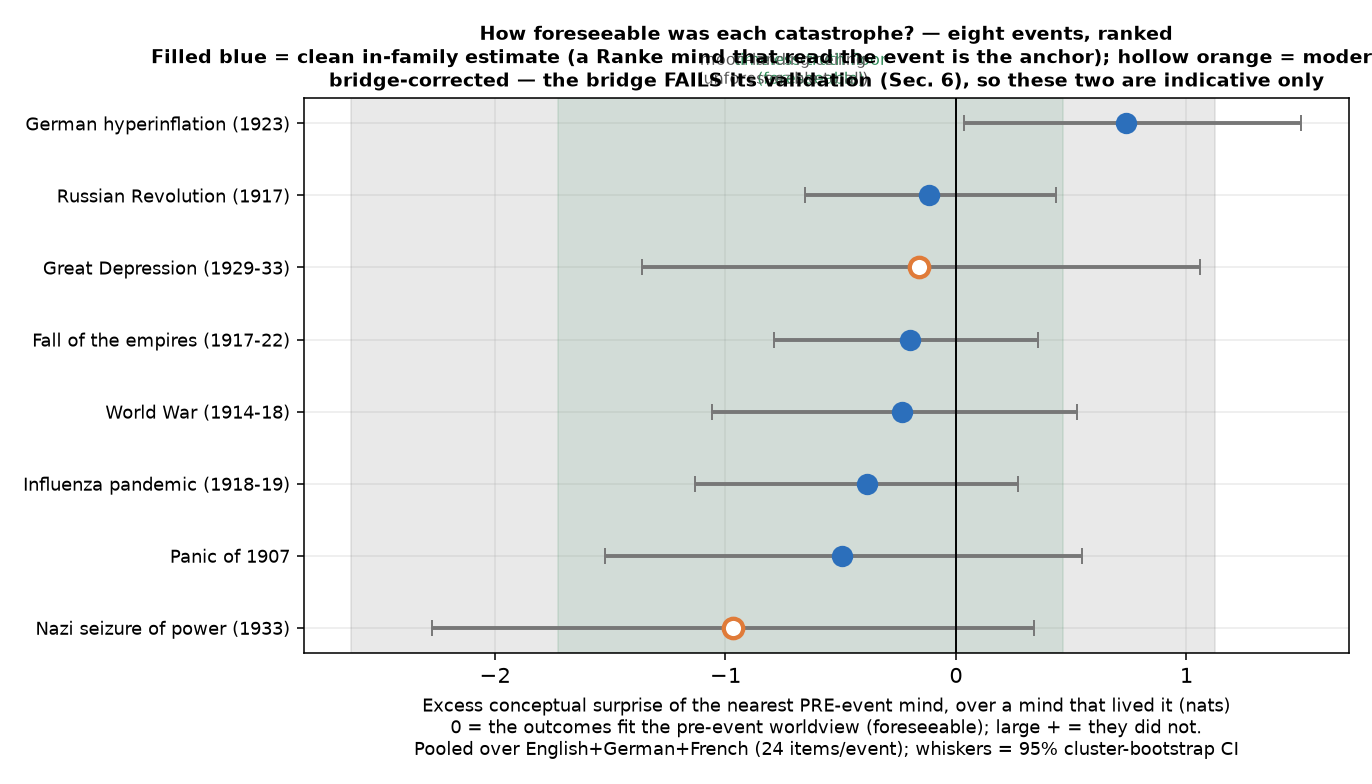
\includegraphics[width=.94\textwidth]{figP1_ranking.png}
\caption{\textbf{The foreseeability ranking.} The \emph{y-axis} lists the eight catastrophes; the
\emph{x-axis measures} the excess believability-strain $\Delta$ of the nearest pre-event reader over a reader
that lived the event (nats), pooled over English, German, and French (24 items per event); whiskers are 95\%
cluster-bootstrap intervals. Zero means the outcomes fit the pre-event worldview; the green band is the
timeless-truth floor, the grey band the moon-landing ceiling. Filled blue markers are clean in-family
estimates; hollow orange markers (Depression, Nazi seizure) rely on a modern-model benchmark that fails its
audit (Section~\ref{sec:validity}) and are indicative only. \emph{Take-away:} panic, war, imperial collapse,
revolution, and pandemic were thinkable in advance; the one in-family event above the floor is the
hyperinflation.}
\label{fig:ranking}
\end{figure}

\begin{table}[t]\centering\small
\begin{tabular}{lccrr}
\toprule
Event & Pre mind & Anchor & $\Delta_{\text{conc}}$ (pooled) & 95\% CI \\
\midrule
Nazi seizure of power (1933) & 1929 & modern (bridged) & $-0.97$ & $[-2.27,\,+0.34]$ \\
Panic of 1907 & 1900 & 1913 (in-family) & $-0.49$ & $[-1.52,\,+0.55]$ \\
Influenza pandemic (1918-19) & 1913 & 1929 (in-family) & $-0.39$ & $[-1.13,\,+0.27]$ \\
World War (1914-18) & 1913 & 1929 (in-family) & $-0.23$ & $[-1.06,\,+0.52]$ \\
Fall of the empires (1917-22) & 1913 & 1929 (in-family) & $-0.20$ & $[-0.79,\,+0.35]$ \\
Great Depression (1929-33) & 1929 & modern (bridged) & $-0.16$ & $[-1.36,\,+1.06]$ \\
Russian Revolution (1917) & 1913 & 1929 (in-family) & $-0.12$ & $[-0.66,\,+0.43]$ \\
German hyperinflation (1923) & 1913 & 1929 (in-family) & $+0.74$ & $[+0.04,\,+1.50]$ \\
\bottomrule
\end{tabular}
\caption{\textbf{The panel, ranked by pooled $\Delta$ at the nearest pre-event reader.} An in-family anchor is
a Ranke model whose corpus contains the event; ``modern (bridged)'' rows are indicative only. Twelve items per
event per language; 95\% cluster-bootstrap intervals over translated item triplets. Per-language estimates in
Appendix~\ref{app:lang}.}
\label{tab:ranking}
\end{table}

Three checks anchor the reading. The 1907 panic --- the pre-registered positive control --- reads at the floor
($\Npanpanic$), as a sound measure must. Twenty-four items carried over verbatim from an earlier battery
reproduce their scores to the second decimal: the pipeline did not move. And the future-to-all controls read
$\approx 0$ \emph{in-family} --- the 1913 and 1929 readers are equally ignorant of the moon --- as designed.

The substantive result is the flatness. The World War at $\Npanwwi$; the fall of the empires at $\Npanemp$;
the revolution at $\Npanrev$; the pandemic at $\Npanflu$: every confidence interval straddles zero, in
English, German, and French alike. These are the events historiography paints as bolts from the blue, and
the minds that preceded them --- certified ignorant of the facts by the gate --- find their outcomes as easy
to believe as the turning of the tides. The empires make the point most sharply: that the Hohenzollern,
Romanov, Habsburg, and Ottoman crowns would all fall was, to the reading public of 1913, in no language a
strange idea.

\subsection{The exception: the death of money}\label{sec:infl}

One in-family event rises above the floor: the hyperinflation, at $\Npaninfl$ nats pooled --- odds understated
roughly $\NoddsInfl$-fold --- the only event whose interval clears zero. The fine print matters. The signal is
French ($\NpaninflFR$ nats, permutation $p=\NpaninflPFR$ against the French floor, the only event-language
cell to survive the false-discovery correction) and German ($\NpaninflDE$); \emph{English readers find even
the death of money thinkable} ($\NpaninflEN$). No single item drives the estimate (largest leave-one-out
shift, $0.46$ nats).

We offer the interpretation as conjecture. Monetary catastrophe was a standing \emph{argument} of the
English-language record --- assignats, greenbacks, the silver agitation, the quantity theorists --- while a
French reader of 1913 had lived five generations inside the franc germinal, untouched since 1803
\citep{keynes1923}. What a worldview can think, the pattern suggests, is what its library kept arguing about.
Section~\ref{sec:selection} shows the same principle governing the misses.

\section{Result II: selection failed --- forecasting by the last precedent}\label{sec:selection}

Support is not selection. For each event, six duels confront the outcome that happened with an equally
dramatic counterfactual that did not, scored as the pre-event reader's calibrated preference; a measure that
merely rewarded catastrophic language would be indifferent, and a mind in the grip of the wrong theory
prefers the counterfactual. (Duels whose neutral frame retains the event identity have little power by
construction; Appendix~\ref{app:duels} codes each duel's informativeness, and the text discusses the
informative set.)

\begin{figure}[t]\centering
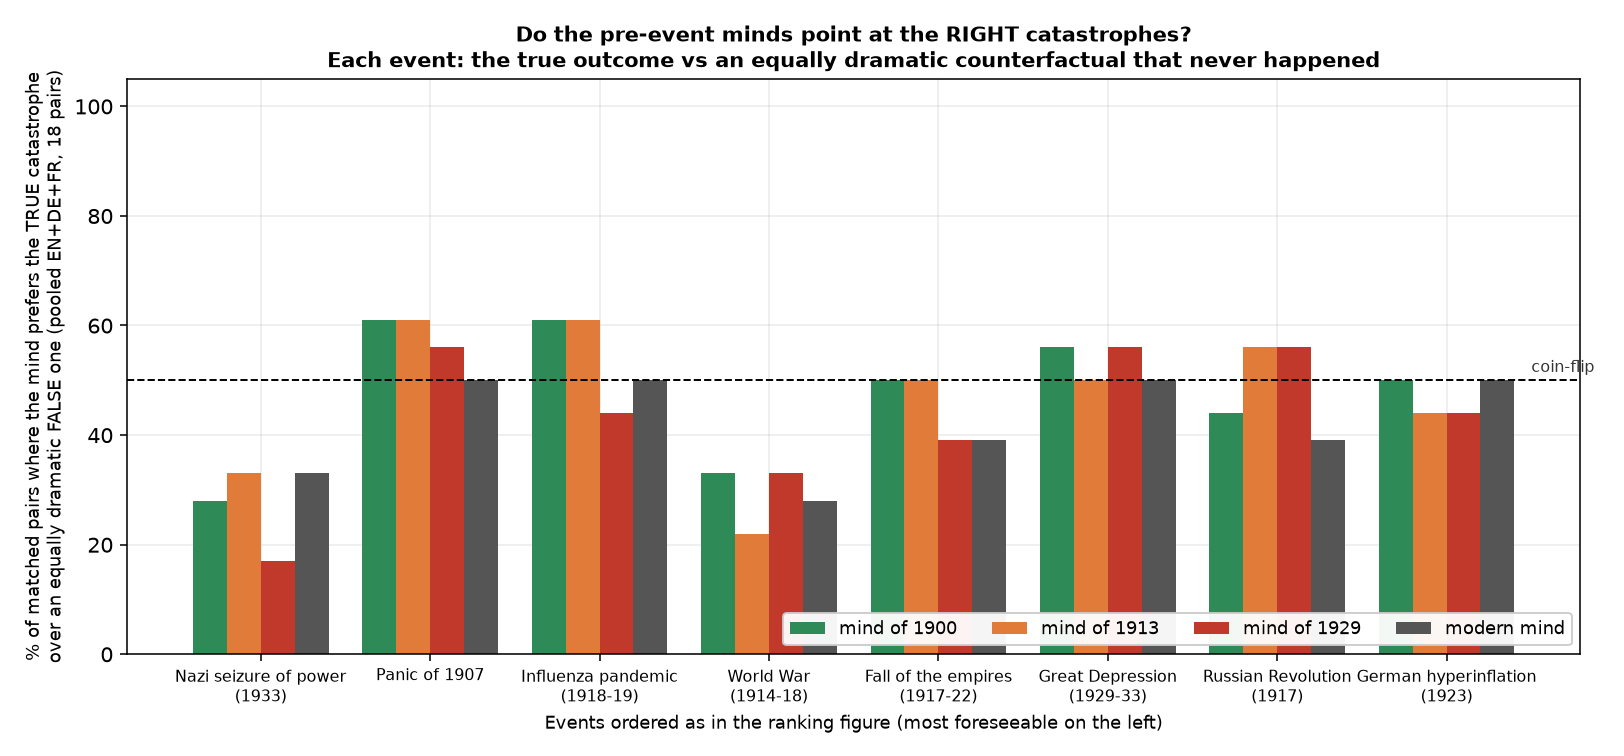
\includegraphics[width=.97\textwidth]{figP3_truefalse.png}
\caption{\textbf{Do the frozen readers point at the right catastrophes?} The \emph{x-axis} lists the events,
ordered as in the ranking; the \emph{y-axis measures} the share of duels in which each reader prefers the
true catastrophe over the matched counterfactual (pooled over languages, 18 duels per event); the dashed line
is a coin flip. Bars are the readers of 1900, 1913, 1929, and a modern model. \emph{Take-away:} the pre-event
readers beat the coin where catastrophe was a recurring genre, and fall below it where the event broke with
precedent --- most severely for the Nazi seizure.}
\label{fig:tf}
\end{figure}

Three events tell the story. The \emph{panic} rewards the 1900 reader ($\Ntfpanicpre$\% of duels): it knows
the trust companies fall first ($\NtfPanicTrusts$ nats) and that the break will be severe
($\NtfPanicSevere$). The \emph{pandemic} splits exactly along the line of precedent: the 1913 reader prefers
``a form of the familiar influenza'' to ``the cholera come again'' ($\NtfFluFormPre$) and places the
pestilence in the last year of the war ($\NtfFluWaryearPre$) --- but bets it will spare the young
($\NtfFluYoungPre$) and that a serum will arrive in time ($\NtfFluSerumPre$). And the \emph{Nazi seizure}
inverts the coin ($\Ntfnazipre$\%, mean margin $\Ntfnazimargin$ nats): the 1929 reader bets against lawful
appointment and for the armed march ($\NtfNaziLawful$), against the corporal and for the generals restoring
the Kaiser ($\NtfNaziCorporal$), against the aged president appointing the man he despised
($\NtfNaziPresident$), against cheering crowds and for civil war ($\NtfNaziCheering$).

\begin{table}[t]\centering\small
\begin{tabular}{p{4.6cm}p{5.6cm}r}
\toprule
The miss & The precedent the mind reached for & Margin (nats) \\
\midrule
The next plague: cholera, not influenza & Hamburg, 1892 --- the last great epidemic \citep{evans1987} & volunteered 6/6$^{a}$ \\
The plague will spare the young & Every prior epidemic killed the weak & $\NtfFluYoungPre$ \\
A serum will conquer it in time & Diphtheria antitoxin, 1894 --- serum triumphalism & $\NtfFluSerumPre$ \\
Power falls to an armed march & Kapp 1920, Munich 1923 --- the putsch template & $\NtfNaziLawful$ \\
The generals restore the Kaiser & The restoration talk of 1918--25 & $\NtfNaziCorporal$ \\
Dictatorship only after civil war & 1919 --- Germany's last descent into street war & $\NtfNaziCheering$ \\
A panic is met with government paper & The greenback and free-silver agitation & $\NtfPanicFinanciers$ \\
\bottomrule
\end{tabular}
\caption{\textbf{Forecasting by the last precedent.} Each row is a duel the pre-event reader loses (negative
margin = prefers the counterfactual), paired with the historical template that counterfactual reapplies.
$^{a}$The cholera row is from free generation: prompted for the next world-sweeping pestilence, the frozen
readers volunteer influenza in $\NprodFluFormTh$ of completions --- the greedy completion names cholera and
cites 1892.}
\label{tab:analogy}
\end{table}

Table~\ref{tab:analogy} names the pattern. Every miss is the most recent precedent, reapplied: the last
epidemic, the last coup, the last monetary agitation. Free generation --- the sternest test, in which the
frozen readers write their own forecasts --- shows the same asymmetry. The 1913 reader \emph{volunteers} the
Tsar's deposition after a lost war ($\NprodRevTsarTh$ of completions: ``be deposed and his son made
Emperor''), and the 1900 reader volunteers suspended payments in a panic ($\NprodPanicBanksNn$); but no
reader, in any completion, volunteers influenza as the next plague ($\NprodFluFormTh$), the death of the
mark ($\NprodInflMarkTh$), or the corporal ($\NprodNaziWhoTN$ --- ``not yet in sight'').

This is the availability heuristic \citep{tversky1973}, measured in the collective text of an era rather
than in a laboratory --- and it is the distortion that diagnostic-expectations models place at the center of
credit booms and busts \citep{bordalo2018,gennaioli2018}: beliefs formed by over-sampling what memory serves
up. In our data the mechanism governs \emph{tails}: societies imagine their disasters by rerunning their most
recent one, so the probability mass sits on the wrong member of the support. Crucially, the same mechanism
explains where foresight \emph{works} --- panics were selected correctly because the precedent happened to be
the right template. Availability is not a bias about drama; it is a bias toward the shelf's newest volume.

\section{Audits}\label{sec:validity}

\paragraph{The gate (A2).} For every event, in every language, six post-event factual probes --- four-way
calibrated forced choice, chance 25\% --- run under the event's pre-event reader; the same probes run under
the anchor certify that hindsight can answer them (the World-War probes are answered 14/15 by the 1929
reader). Seven of eight events gate GREEN (Table~\ref{tab:gates}): the reader that finds the pandemic easy
to believe cannot name it, date it, or count its dead. The one AMBER --- the revolution --- dissolves on
inspection into a geography prior: the 1913 reader aces only the fortress-town item (``peace signed at
Brest-Litovsk,'' 3/3) while flooring on Lenin (0/3), the party (1/3), and the month (1/3); excluding that
item post hoc gives $\Ngaterevposthoc$ ($p=\NgaterevposthocP$), consistent with chance. The registered
verdict stands, and the caveat travels with the revolution's estimate.

\begin{table}[t]\centering\small
\begin{tabular}{lcllll}
\toprule
Event & Pre mind & Gate (pre) & correct & Ceiling & correct \\
\midrule
Panic of 1907 & 1900 & GREEN & 3/15 & OK & 10/15 \\
World War (1914-18) & 1913 & GREEN & 7/15 & OK & 14/15 \\
Fall of the empires (1917-22) & 1913 & GREEN & 7/15 & OK & 8/15 \\
Russian Revolution (1917) & 1913 & AMBER$^{\dagger}$ & 9/18 & OK & 10/18 \\
Influenza pandemic (1918-19) & 1913 & GREEN & 6/18 & OK & 9/18 \\
German hyperinflation (1923) & 1913 & GREEN & 5/18 & OK & 11/18 \\
Great Depression (1929-33) & 1929 & GREEN & 5/15 & OK & 12/15 \\
Nazi seizure of power (1933) & 1929 & GREEN & 5/18 & WEAK-PROBES & 8/18 \\
\bottomrule
\end{tabular}
\caption{\textbf{The contamination gate.} GREEN = pre-event accuracy consistent with chance (binomial test):
the low strain of Section~\ref{sec:thinkable} is foresight, not leakage. The ceiling column validates the
probes under the hindsight anchor. Items with pre-registered period-prior caveats are excluded from verdicts.
$^{\dagger}$Post-hoc sensitivity discussed in the text.}
\label{tab:gates}
\end{table}

\paragraph{The offset audit (why in-family).} Whatever the 1929 reader's strain, relative to a modern model,
on events its corpus \emph{contains} cannot be foresight failure. Measured across five such events, that
offset is $\NpanoffsetEN$/$\NpanoffsetDE$/$\NpanoffsetFR$ nats (English/German/French): the 1929 reader
``fails to foresee'' the World War it lived through by $\NwwiXSatTNEN$ nats against a modern benchmark. The
offset is also content-dependent --- after subtracting it, the moon landing reads $\NtripCrawDE$ nats in
German, an absurdity traceable to control items whose archaic phrasing the modern model itself finds strained
--- so no constant correction rescues cross-family comparison. Everything that carries weight in this paper is
in-family.

\paragraph{Placebos and mechanics.} The timeless-truth floor and moon ceiling reproduce per language
(Table~\ref{tab:ranking} notes; Appendix~\ref{app:lang}); no pre-1930 reader finds any future-to-all item
easy against the in-family anchor (the leak tripwire); leave-one-out influence and the false-discovery
correction are reported for every estimate (Appendix~\ref{app:lang}); and the same-tokenizer decomposition
of raw surprise into word-novelty and idea-novelty --- the mechanics established in our English-bank study,
where the World War's raw surprise of $\NwwidSTh$ nats proves $\NwwiDlexTh$ words and $\NwwiDconcTh$ idea ---
is summarized in Appendix~\ref{app:english}.

\section{The Great Depression: a bracketed verdict}\label{sec:depression}

The literature's central case lacks what our method needs --- a frozen reader who lived through it. We
therefore report a bracket, and we can say precisely why the bracket's ends differ.

The case that the Depression was a true outlier rests on two offset-free instruments. Within the 1929
reader, Depression outcomes exceed World-War outcomes --- an event that reader lived through --- by
$\NcontrastDiff$ nats (95\% CI $\NcontrastCI$, $p=\NcontrastP$): roughly an $\NoddsHeadline$-fold difference
in relative odds, produced by a mind the gate certifies clean on Depression facts (and on the crash itself).
And genuine period prose, which involves no constructed sentences, agrees: with the author held fixed across
the shock (Keynes and Angell; Hoover and Roosevelt), Depression-era text stays foreign to every pre-1930
reader ($\NtextDepDiDTN$ nats per character at the 1929 reader, CI $\NtextDepCiTN$) while World-War text
passes its own control ($\NtextWWIdidTh$, CI $\NtextWWIciTh$).

The case against comes from the panel's own Depression battery, whose bridged estimate is $\Npandep$ ---
nothing. We can localize the disagreement. It is not item content: on six outcome statements present in both
banks --- the crash from the plateau, one man in four idle, banks failing by the thousand --- the English-bank
instrument reads $\NdepMatchedVOne$ nats and the panel instrument reads $\NdepMatchedPanel$. It is the
\emph{calibration frame}: the English bank de-loads its baseline deeply (generic subjects), the panel lightly
(the item's own subject, stripped of the scenario) --- and a light baseline absorbs part of the event into
the benchmark. Nor is it severity: classifying every Depression item by whether its outcome quantifies a
magnitude outside pre-1914 experience, severity items show \emph{no} excess over genre items in either bank
($\NdepSevGenDiff$ in the English bank; Appendix~\ref{app:decomp}) --- the ``foreseeable in kind,
unforeseeable in magnitude'' resolution, attractive as it sounds, is not in the data.

Where does that leave 1929? Two instruments of three --- including the only one that uses no constructed
language at all --- find a genuine Depression excess; the most conservative finds none; all three agree the
excess, if real, is unlike anything else in the panel. We read the weight of evidence as favoring Depression
exceptionalism, hold the magnitude open, and note that the question is closable: a frozen reader trained to
1938 would anchor both post-1929 events in-family, and the machinery of this paper would settle in an
afternoon what the historiography has argued for ninety years.

\section{What the measurements change}\label{sec:implications}

\paragraph{For disaster-risk models.} Return to \citet{barro2006}. The rare-disaster resolution of the
equity-premium puzzle calibrates a disaster probability from the realized twentieth century and attributes
it, ex ante, to investors. Our measurements speak to both halves of that move. The \emph{support} assumption
survives handsomely: we find no catastrophe --- war, imperial collapse, revolution, pandemic --- that the
pre-event record could not generate; the ``unimaginable disaster'' defense of low pre-1914 risk premia is
not available, and on this point the calibrations are vindicated against their historiographical critics.
The \emph{weights} assumption does not survive: the same readers misallocate probability across the support
by factors of two to seven, always toward the most recent precedent. The July-1914 bond puzzle
\citep{ferguson2006} then needs no unimaginability --- investors could think the war; they weighted the
wrong futures --- and models of \emph{time-varying} disaster premia \citep{gabaix2012,wachter2013} acquire a
measurable state variable: perceived tail risk should load on the recency and salience of precedent, and
time-locked readers make that loading estimable decade by decade. For the peso-problem tradition
\citep{krasker1980}, the method supplies the missing observable: the state that is in minds but not in
samples can now be read out of the minds directly.

\paragraph{For the economics of beliefs.} Diagnostic-expectations theory \citep{bordalo2018,gennaioli2018}
was built on laboratory heuristics \citep{tversky1973} and validated on modern survey and credit-cycle data.
Our duels supply something the field has lacked: evidence that the same memory-driven distortion governed
the \emph{tail beliefs of whole societies}, a century before the surveys, with the distorting precedent
identifiable event by event --- Hamburg 1892 for the pandemic, the putsches of 1920--23 for the seizure of
power. Belief formation by availability is not a modern artifact of financial markets; it is how the written
record itself weighs futures.

\paragraph{For historical method.} Every debate about hindsight --- from the sleepwalkers of 1914 to the
black swans of finance \citep{taleb2007,tetlock2005,kuran1991} --- turns on an unobservable: what the past
could have known. Time-locked readers make that counterfactual estimable under stated assumptions, with
audits (contamination gates, placebo duels, in-family anchoring) that we expect to travel to any question of
the same form. The instrument is general; 1907--1933 was only its first assignment.

\section{Conclusion}\label{sec:conclusion}

Foreseeability can be measured, and for the early twentieth century the measurement reverses the cliché
twice. The catastrophes were not unthinkable: to certified-ignorant readers of 1900 and 1913, in three
languages, the panic, the war, the end of the empires, the revolution, and the pandemic read like weather ---
only the death of money strained the worldview, and only where the library had never argued about it. But
thinkable was not chosen: asked to weigh true futures against false ones, the same readers reached for the
newest precedent on the shelf and bet, again and again, on the wrong volume --- most catastrophically in
1933, when every duel favored a putsch that never came over the appointment that did. The failure of the age
was not imagination. It was selection --- and selection failed in a way that was systematic, textual, and,
we now know, measurable in advance.

\begin{thebibliography}{99}
\bibitem[Angell(1910)]{angell1910} Angell, Norman. 1910. \emph{The Great Illusion}. London: Heinemann.
\bibitem[Bagehot(1873)]{bagehot1873} Bagehot, Walter. 1873. \emph{Lombard Street: A Description of the Money
Market}. London: Henry S. King.
\bibitem[Barro(2006)]{barro2006} Barro, Robert J. 2006. ``Rare Disasters and Asset Markets in the Twentieth
Century.'' \emph{Quarterly Journal of Economics} 121(3): 823--866.
\bibitem[Barro and Urs\'ua(2008)]{barroursua2008} Barro, Robert J., and Jos\'e F. Urs\'ua. 2008.
``Macroeconomic Crises since 1870.'' \emph{Brookings Papers on Economic Activity} 39(1): 255--350.
\bibitem[Barry(2004)]{barry2004} Barry, John M. 2004. \emph{The Great Influenza}. New York: Viking.
\bibitem[Bloch(1899)]{bloch1899} Bloch, Ivan S. 1899. \emph{Is War Now Impossible?} London: Grant Richards.
\bibitem[Bordalo et al.(2018)]{bordalo2018} Bordalo, Pedro, Nicola Gennaioli, and Andrei Shleifer. 2018.
``Diagnostic Expectations and Credit Cycles.'' \emph{Journal of Finance} 73(1): 199--227.
\bibitem[Bruner and Carr(2007)]{bruner2007} Bruner, Robert F., and Sean D. Carr. 2007. \emph{The Panic of
1907}. Hoboken: Wiley.
\bibitem[Clark(2012)]{clark2012} Clark, Christopher. 2012. \emph{The Sleepwalkers: How Europe Went to War in
1914}. London: Allen Lane.
\bibitem[Crosby(1989)]{crosby1989} Crosby, Alfred W. 1989. \emph{America's Forgotten Pandemic: The Influenza
of 1918}. Cambridge: Cambridge University Press.
\bibitem[Evans(1987)]{evans1987} Evans, Richard J. 1987. \emph{Death in Hamburg: Society and Politics in the
Cholera Years}. Oxford: Oxford University Press.
\bibitem[Evans(2003)]{evans2003} Evans, Richard J. 2003. \emph{The Coming of the Third Reich}. London: Allen
Lane.
\bibitem[Feldman(1993)]{feldman1993} Feldman, Gerald D. 1993. \emph{The Great Disorder: Politics, Economics,
and Society in the German Inflation, 1914--1924}. New York: Oxford University Press.
\bibitem[Ferguson(2006)]{ferguson2006} Ferguson, Niall. 2006. ``Political Risk and the International Bond
Market between the 1848 Revolution and the Outbreak of the First World War.'' \emph{Economic History Review}
59(1): 70--112.
\bibitem[Fergusson(1975)]{fergusson1975} Fergusson, Adam. 1975. \emph{When Money Dies}. London: Kimber.
\bibitem[Fisher(1930)]{fisher1930} Fisher, Irving. 1930. \emph{The Stock Market Crash---and After}. New
York: Macmillan.
\bibitem[Friedman and Schwartz(1963)]{friedman1963} Friedman, Milton, and Anna J. Schwartz. 1963. \emph{A
Monetary History of the United States, 1867--1960}. Princeton: Princeton University Press.
\bibitem[Gabaix(2012)]{gabaix2012} Gabaix, Xavier. 2012. ``Variable Rare Disasters: An Exactly Solved
Framework for Ten Puzzles in Macro-Finance.'' \emph{Quarterly Journal of Economics} 127(2): 645--700.
\bibitem[Galbraith(1955)]{galbraith1955} Galbraith, John Kenneth. 1955. \emph{The Great Crash, 1929}.
Boston: Houghton Mifflin.
\bibitem[Gennaioli and Shleifer(2018)]{gennaioli2018} Gennaioli, Nicola, and Andrei Shleifer. 2018. \emph{A
Crisis of Beliefs: Investor Psychology and Financial Fragility}. Princeton: Princeton University Press.
\bibitem[Gentzkow et al.(2019)]{gentzkow2019} Gentzkow, Matthew, Bryan Kelly, and Matt Taddy. 2019. ``Text
as Data.'' \emph{Journal of Economic Literature} 57(3): 535--574.
\bibitem[Hoover(1929)]{hoover1929} Hoover, Herbert. 1929. Inaugural Address, March 4, 1929.
\bibitem[Keynes(1919)]{keynes1919} Keynes, John Maynard. 1919. \emph{The Economic Consequences of the
Peace}. London: Macmillan.
\bibitem[Keynes(1923)]{keynes1923} Keynes, John Maynard. 1923. \emph{A Tract on Monetary Reform}. London:
Macmillan.
\bibitem[Kindleberger(1973)]{kindleberger1973} Kindleberger, Charles P. 1973. \emph{The World in Depression,
1929--1939}. Berkeley: University of California Press.
\bibitem[Krasker(1980)]{krasker1980} Krasker, William S. 1980. ``The `Peso Problem' in Testing the
Efficiency of Forward Exchange Markets.'' \emph{Journal of Monetary Economics} 6(2): 269--276.
\bibitem[Kuran(1991)]{kuran1991} Kuran, Timur. 1991. ``Now Out of Never: The Element of Surprise in the East
European Revolution of 1989.'' \emph{World Politics} 44(1): 7--48.
\bibitem[Rietz(1988)]{rietz1988} Rietz, Thomas A. 1988. ``The Equity Risk Premium: A Solution.''
\emph{Journal of Monetary Economics} 22(1): 117--131.
\bibitem[Roosevelt(1933)]{roosevelt1933} Roosevelt, Franklin D. 1933. First Inaugural Address, March 4, 1933.
\bibitem[Taleb(2007)]{taleb2007} Taleb, Nassim Nicholas. 2007. \emph{The Black Swan}. New York: Random House.
\bibitem[Tetlock(2005)]{tetlock2005} Tetlock, Philip E. 2005. \emph{Expert Political Judgment}. Princeton:
Princeton University Press.
\bibitem[Tuchman(1962)]{tuchman1962} Tuchman, Barbara W. 1962. \emph{The Guns of August}. New York:
Macmillan.
\bibitem[Turner(1996)]{turner1996} Turner, Henry Ashby. 1996. \emph{Hitler's Thirty Days to Power: January
1933}. Reading, MA: Addison-Wesley.
\bibitem[Tversky and Kahneman(1973)]{tversky1973} Tversky, Amos, and Daniel Kahneman. 1973. ``Availability:
A Heuristic for Judging Frequency and Probability.'' \emph{Cognitive Psychology} 5(2): 207--232.
\bibitem[Wachter(2013)]{wachter2013} Wachter, Jessica A. 2013. ``Can Time-Varying Risk of Rare Disasters
Explain Aggregate Stock Market Volatility?'' \emph{Journal of Finance} 68(3): 987--1035.
\bibitem[Zweig(1942)]{zweig1942} Zweig, Stefan. 1942. \emph{The World of Yesterday}. Stockholm:
Bermann-Fischer.
\end{thebibliography}

\clearpage
\appendix
\renewcommand{\thesection}{\Alph{section}}
\section*{Appendix}

\section{The bank: construction, screens, freeze}\label{app:bank}
The full item bank --- $\Nitems$ English-bank items plus the panel's 96 event items, 33 controls, 48 duels,
and 48 gate probes, each in three languages --- is in the replication repository
(\texttt{results/question\_bank\_panel.json}, SHA-256 hashed at freeze), together with the automated screen
report: structure checks, target-in-stem leakage, cross-language length parity ($\le 2.0\times$ in
characters), and a period-vocabulary screen that scores every stem under the 1913 model itself and flags
robust outliers. The pre-registration (\texttt{docs/PREREGISTRATION\_FORESIGHT\_v2.md}) locks estimators,
hypotheses --- including the panic-as-positive-control prediction and the bridge validation requirement ---
exclusion rules, and statistics before scoring. The transparent report
(\texttt{reports/panel\_events.html}) lists every prompt, every neutral frame, every duel, and every score.

\section{Gates in full}\label{app:gates}
Per-item, per-language gate results, including the four pre-registered period-prior exclusions (Morgan,
Versailles, Franz Ferdinand, Roosevelt), the revolution's Brest-Litovsk post-hoc sensitivity
($\Ngaterevposthoc$, $p=\NgaterevposthocP$), and the weak ceiling of the Nazi probes under the modern model
(which makes that gate less informative, not the reader less clean) are in
\texttt{results/gate\_panel.json} and \texttt{reports/panel\_events.html}.

\section{Per-language estimates, influence, and multiplicity}\label{app:lang}
\begin{table}[h]\centering\small
\begin{tabular}{lrrr}
\toprule
Event & English & German & French \\
\midrule
Nazi seizure of power (1933) & $+0.25$ & $-2.52$ & $-0.63$ \\
Panic of 1907 & $+0.15$ & $-0.82$ & $-0.81$ \\
Influenza pandemic (1918-19) & $-0.64$ & $+0.04$ & $-0.55$ \\
World War (1914-18) & $-0.77$ & $-0.45$ & $+0.53$ \\
Fall of the empires (1917-22) & $-0.58$ & $-0.03$ & $+0.01$ \\
Great Depression (1929-33) & $+0.55$ & $-1.67$ & $+0.64$ \\
Russian Revolution (1917) & $-0.69$ & $+1.18$ & $-0.83$ \\
German hyperinflation (1923) & $-0.12$ & $+0.95$ & $+1.39$ \\
\midrule
Timeless-truth floor & $-0.92$ & $+0.16$ & $-1.43$ \\
Moon-landing ceiling & $+0.82$ & $-2.32$ & $-0.05$ \\
\bottomrule
\end{tabular}
\caption{Per-language $\Delta$ at the nearest pre-event reader; floor and ceiling rows on the identical
estimator. Hyperinflation's French estimate ($\NpaninflFR$, $p=\NpaninflPFR$) is the only cell surviving the
Benjamini--Hochberg correction across the eight events; the largest leave-one-out shift for the pooled
hyperinflation estimate is $0.46$ nats. The German ceiling value illustrates the register sensitivity of
cross-family comparison discussed in Section~\ref{sec:validity}.}
\end{table}

\section{The English confirmation study}\label{app:english}
Our registered English-bank study ($\Nitems$ items, two events) established the mechanics the panel scales:
the same-tokenizer split of raw surprise into word-novelty and idea-novelty (the World War's $\NwwidSTh$-nat
raw surprise decomposes into $\NwwiDlexTh$ lexical and $\NwwiDconcTh$ conceptual); the ``home by Christmas''
result (under length-matched forced choice the 1913 reader expects the long war, and volunteers ``for
years'' in free generation, while never volunteering the war's scale in lives); the within-1929 contrast of
Section~\ref{sec:depression}; and the real-prose arm (per-character surprise, author held fixed across the
shock). Full figures and tables: \texttt{reports/walkthrough.html}, \S1--\S7.

\section{Duel informativeness}\label{app:duels}
\begin{table}[h]\centering\small
\begin{tabular}{lrrrr}
\toprule
Event & mind of 1900 & 1913 & 1929 & modern \\
\midrule
Nazi seizure of power (1933) & 28\% & 33\% & 17\% & 33\% \\
Panic of 1907 & 61\% & 61\% & 56\% & 50\% \\
Influenza pandemic (1918-19) & 61\% & 61\% & 44\% & 50\% \\
World War (1914-18) & 33\% & 22\% & 33\% & 28\% \\
Fall of the empires (1917-22) & 50\% & 50\% & 39\% & 39\% \\
Great Depression (1929-33) & 56\% & 50\% & 56\% & 50\% \\
Russian Revolution (1917) & 44\% & 56\% & 56\% & 39\% \\
German hyperinflation (1923) & 50\% & 44\% & 44\% & 50\% \\
\bottomrule
\end{tabular}
\caption{All duel results by reader (share of pairs won by the truth, pooled over languages). Duels whose
neutral frame retains the event identity (most World-War and empire duels) calibrate away the loaded content
and carry little information by construction; the informative duels --- panic, pandemic, Depression, Nazi
seizure --- are those whose counterfactual redirects the catastrophe itself. Per-duel margins:
\texttt{reports/panel\_events.html}.}
\label{tab:tf}
\end{table}

\section{The Depression decomposition}\label{app:decomp}
Classifying every Depression item by a pre-stated rule --- \emph{severity} if the outcome quantifies a
magnitude, duration, or regime break outside pre-1914 business-cycle experience, \emph{genre} otherwise ---
severity items show no excess over genre items in the English bank ($\NdepSevVOne$ vs.\ $\NdepGenVOne$;
difference $\NdepSevGenDiff$) or the panel, and the ordering is robust to recoding the three ambiguous
items. The matched-content frame comparison of Section~\ref{sec:depression} ($\NdepMatchedVOne$ vs.\
$\NdepMatchedPanel$ on identical outcomes) localizes the inter-bank disagreement to calibration-frame depth.

\section{The worldview probes (Zweig)}\label{app:zweig}
A companion battery tests four beliefs Stefan Zweig attributed to the pre-1914 world \citep{zweig1942}:
irresistible progress, the unthinkability of war, the confinement of women, the veneration of age. At full
battery strength (five calibrated belief-versus-skeptic items per theme, three languages), war-unthinkability
survives as a \emph{French} belief ($\NzwiiiwarFR$ nats at 1913; the English reader expects war,
$\NzwiiiwarEN$; the German estimate flips sign with battery size and is not robust); progress is held
everywhere, modestly; women and youth never register. Worldview probes are battery-sensitive in a way the
event panel is not, and we accordingly claim nothing from them beyond the French result. Details:
\texttt{results/zweig\_probe\_v2.json}; \texttt{reports/walkthrough.html} \S8.

\end{document}
